% Results / Parser output
\section{Parser Output / AST}
\label{sect:results:parser_output_ast}
In this section we will present the generated AST output from the generated
parser, and compare them to their respective queries. The results presented here
are discussed in section \ref{sect:discussion:ast}.

\emph{Note: all graphical AST figures in this section were generated using the
actual parser with a custom method to output dot code for the graphviz tool.}

\subsection{FLWOR}
Figure \ref{tree:ast:flwor1} shows the AST generated for the expression in
figure \ref{code:ast:flwor1}. This is a simple example, but it shows one way to
build an AST for a FLWOR expression.

\pagebreak
\begin{figure}[h!]
\verbatiminput{graph_queries/flwor1.xq}
\caption{FLWOR expression example, generates AST seen in figure \ref{tree:ast:flwor1}}
\label{code:ast:flwor1}
\centering
 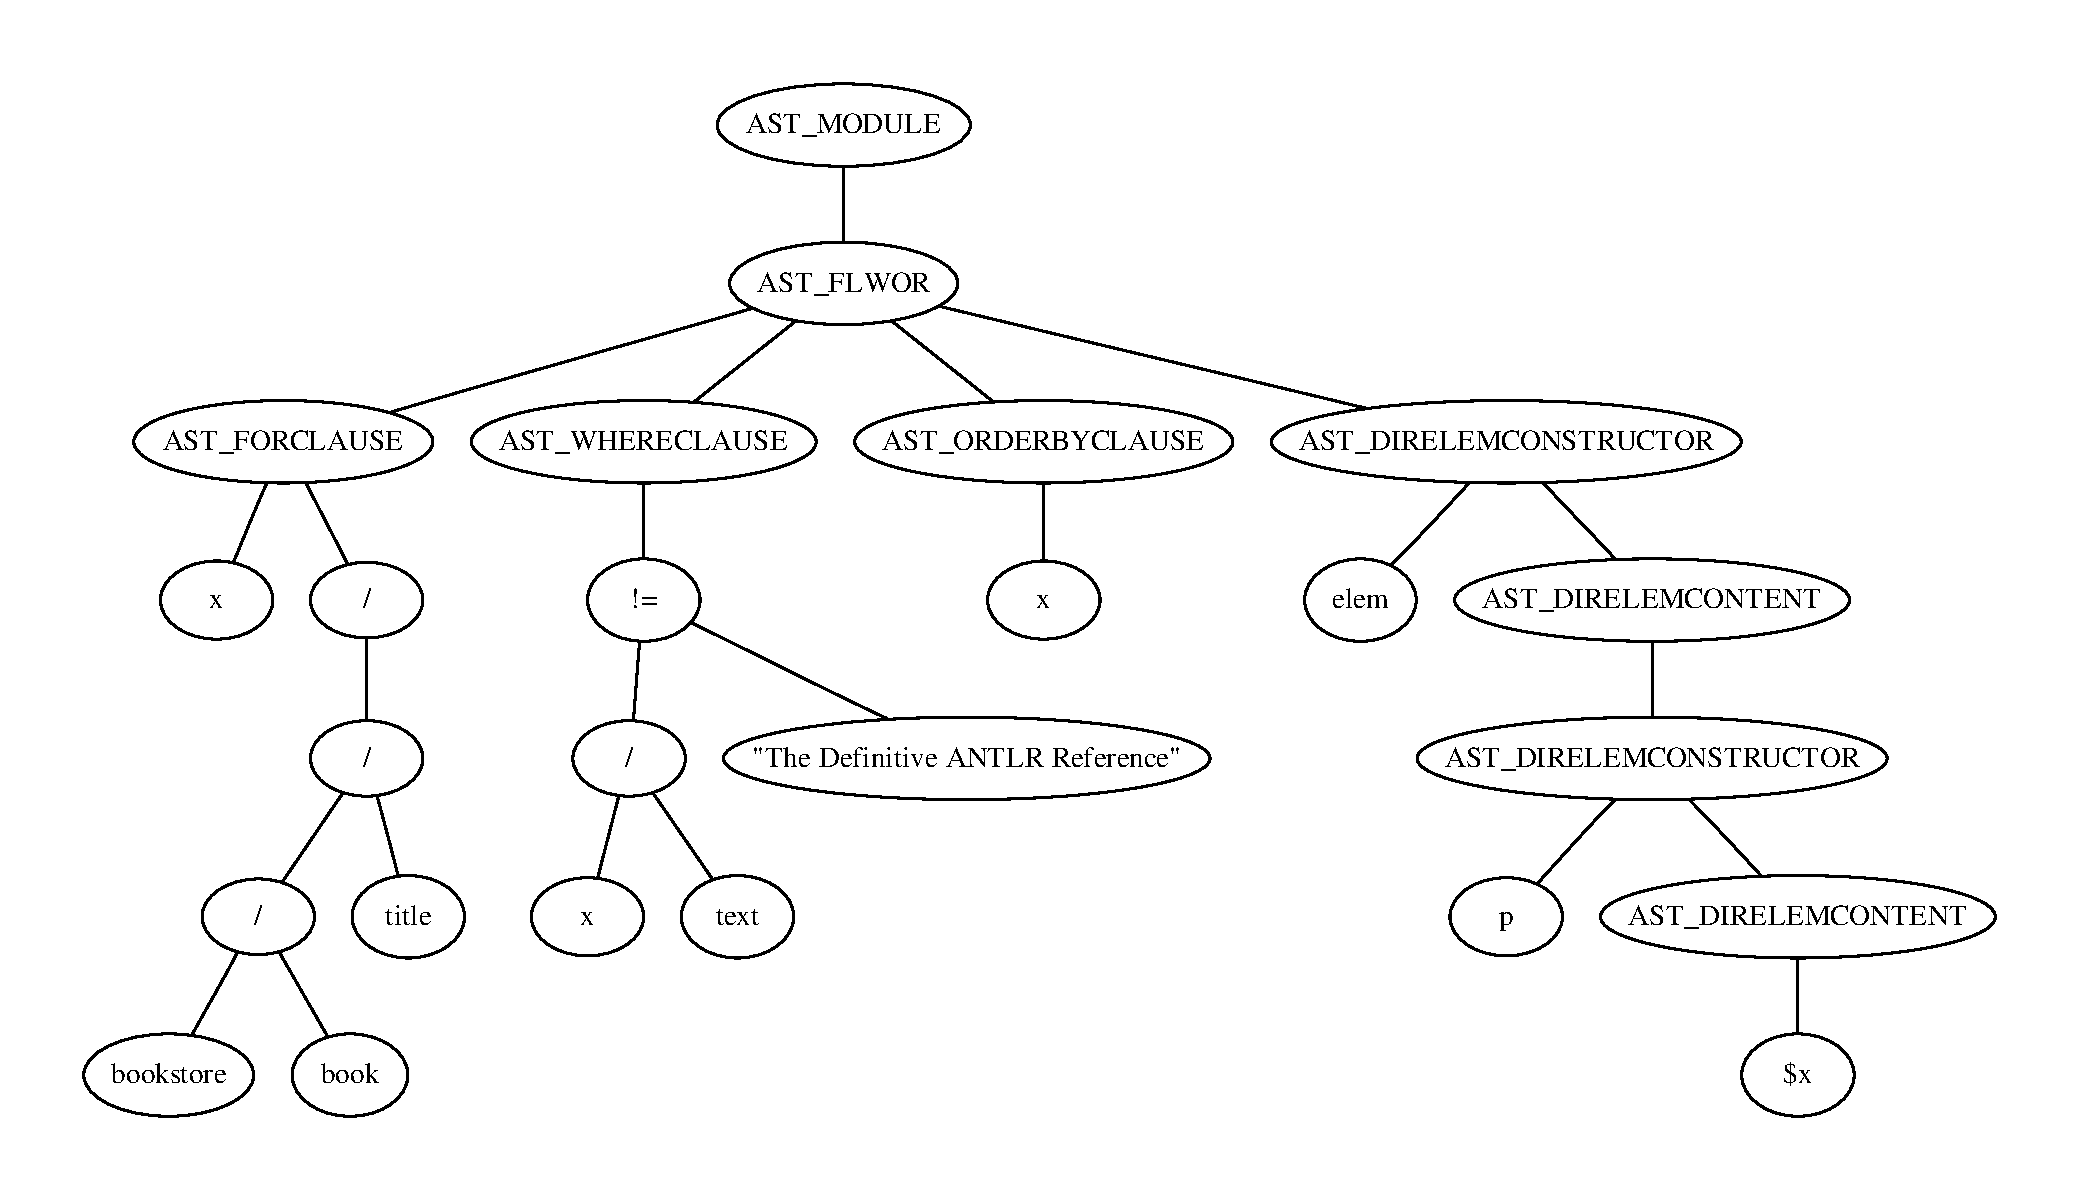
\includegraphics[width=1\textwidth]{img/graphs/flwor1}
\caption{Generated AST tree for FLWOR-expression in figure \ref{code:ast:flwor1}}
\label{tree:ast:flwor1}
\end{figure}

\subsection{Path Expressions}
Figure \ref{tree:ast:pathexpr} shows the AST generated for the query in figure
\ref{tree:ast:pathexpr}. Note that the root node is a single slash with a
single child. Included in this example is also a simple predicate expressions,
illustrating one possible interpretation of this construct.

\pagebreak
\begin{figure}[h!]
\verbatiminput{graph_queries/pathexpr.xq}
\caption{Path expression example, generates AST seen in figure \ref{tree:ast:pathexpr}}
\label{code:xq:pathexpr}
\centering
 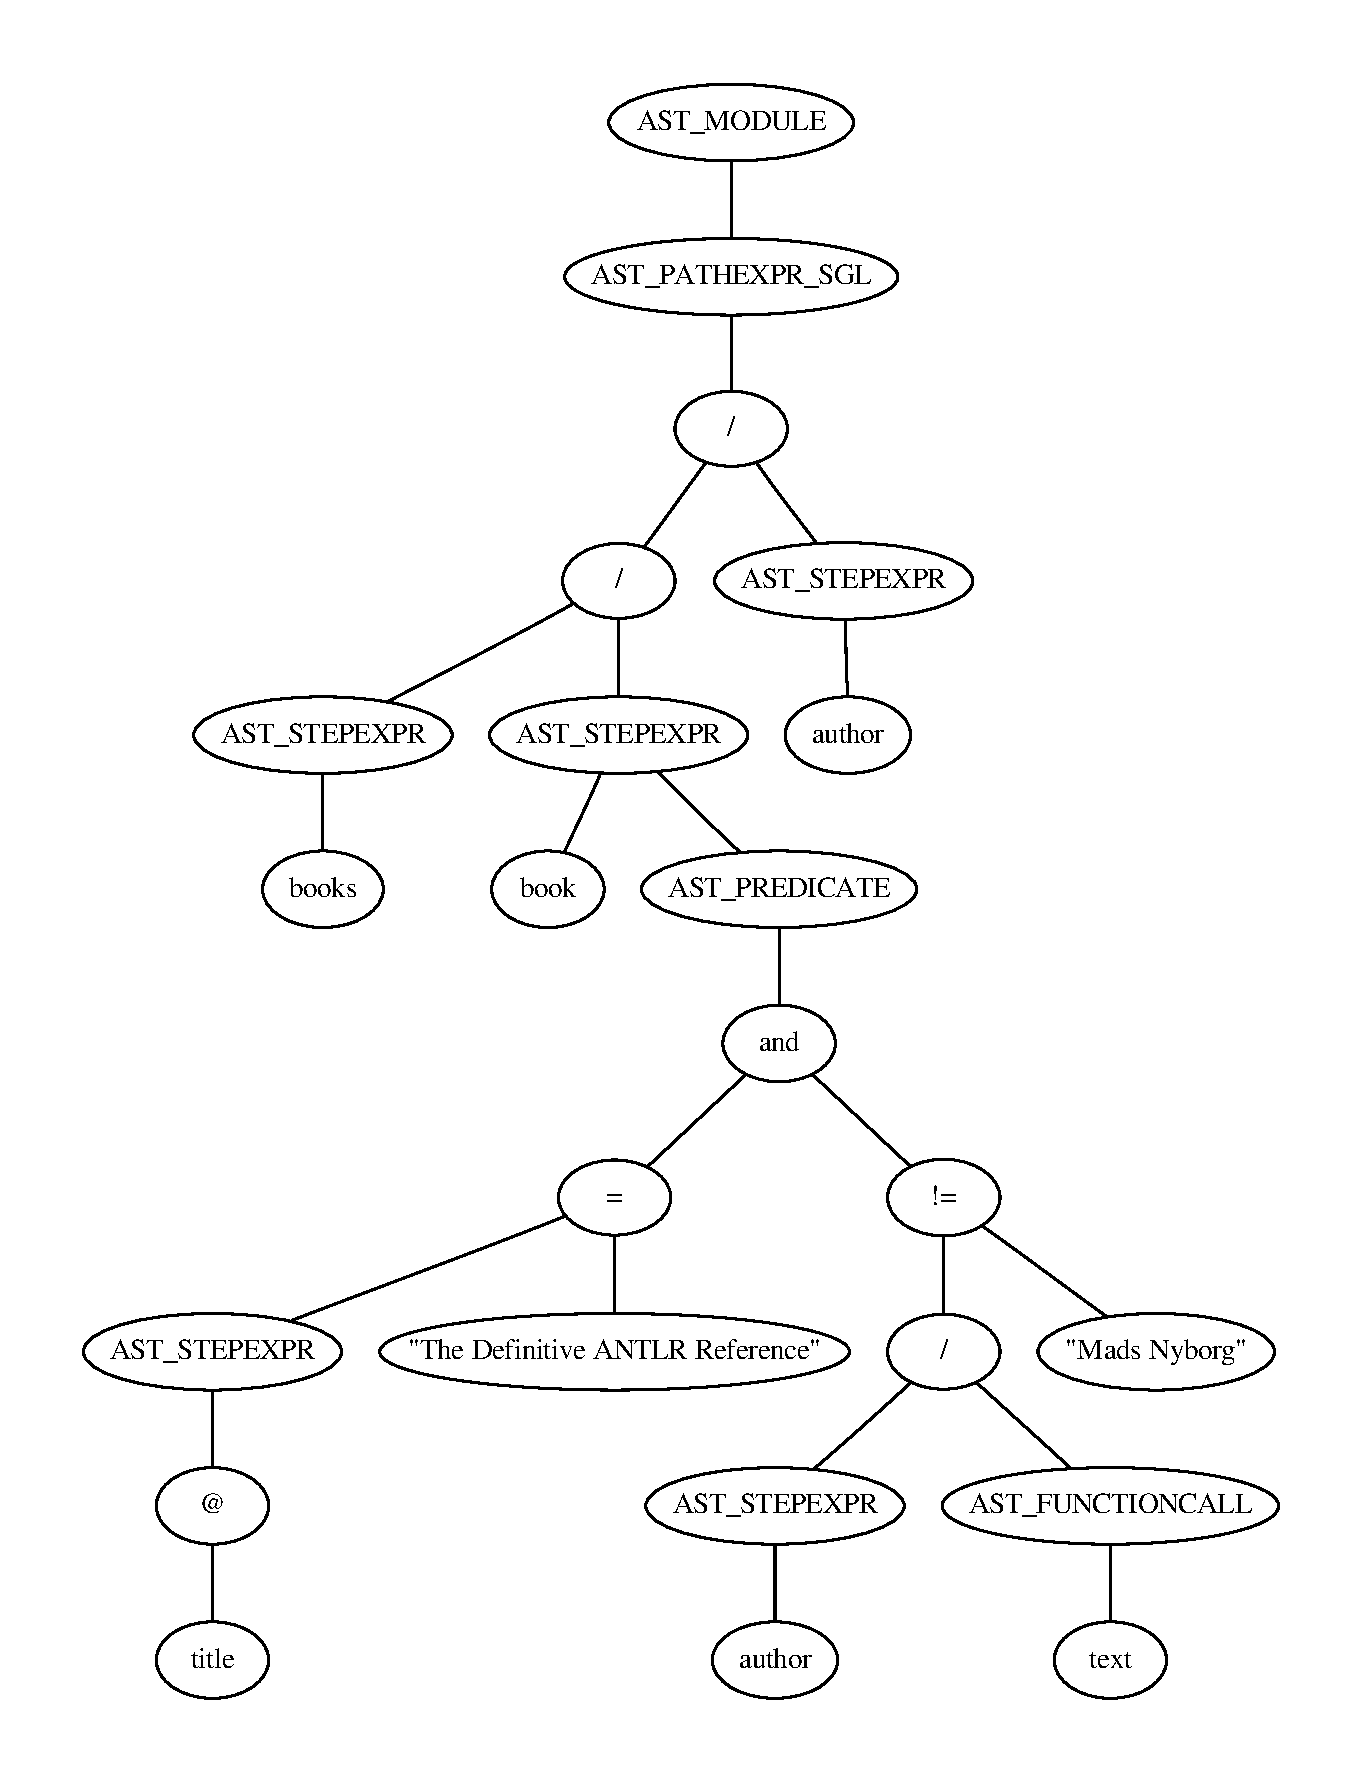
\includegraphics[width=0.8\textwidth]{img/graphs/pathexpr}
\caption{Generated AST tree for the path expression in figure 
\ref{code:xq:pathexpr}}
\label{tree:ast:pathexpr}
\end{figure}

\subsection{Function Declarations}

As seen in figure \ref{code:ast:funcdecl1}, function declarations are aggregated
into a root node (AST\_FUNCTIONDECL) with a function name and optionally
parameters, type, and function body (unless declared as external).

\pagebreak
\begin{figure}[h!]
\verbatiminput{graph_queries/funcdecl1.xq}
\caption{Function declaration used to generate the AST in figure
\ref{tree:ast:funcdecl1}}
\label{code:xq:funcdecl1}
\centering
 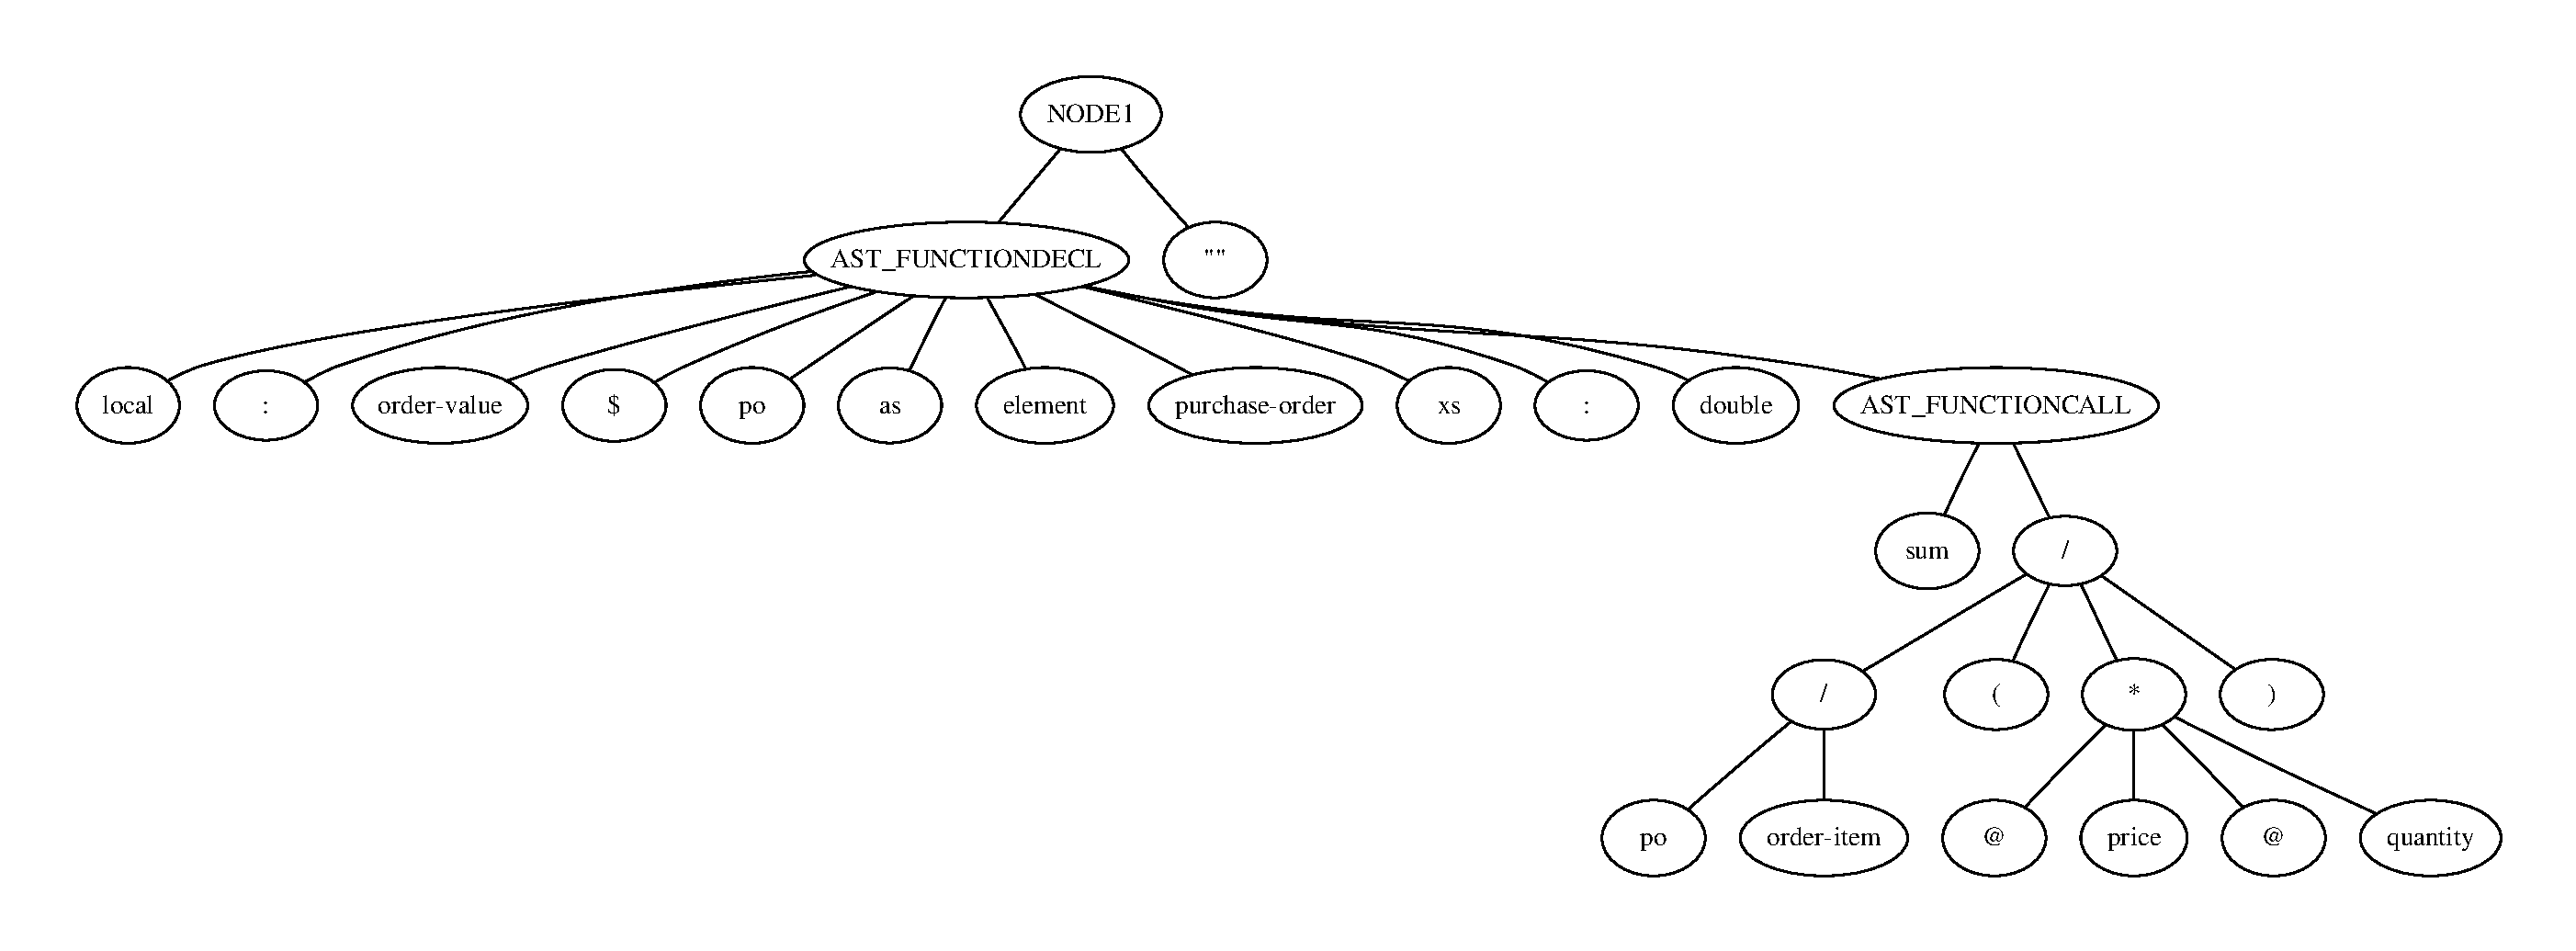
\includegraphics[width=1\textwidth]{img/graphs/funcdecl1}
\caption{Generated AST tree for the function declaration in figure \ref{code:xq:funcdecl1}}
\label{tree:ast:funcdecl1}
\end{figure}

\subsection{Full-Text Operations}
The query in figure \ref{code:xq:ftq1} and the generated AST in figure
\ref{tree:ast:ftq1} shows one possible interpretation of several full-text 
operators in XQuery. In the case of \verb!ftcontains! and \verb!ftand!, this AST
is intuitive, however the interpretation of the \verb!with! operator (as well
as \verb!without! and others) in this example can be done in several other ways.
For example, it may be benefitial to add imaginary tokens to aggregate these
multi-level operator tokens into one single imaginary token.

\begin{figure}[h!]
\verbatiminput{graph_queries/ftq1.xq}
\caption{Full-text XQuery expression used to generate the AST in figure
\ref{tree:ast:ftq1}}
\label{code:xq:ftq1}
\centering
 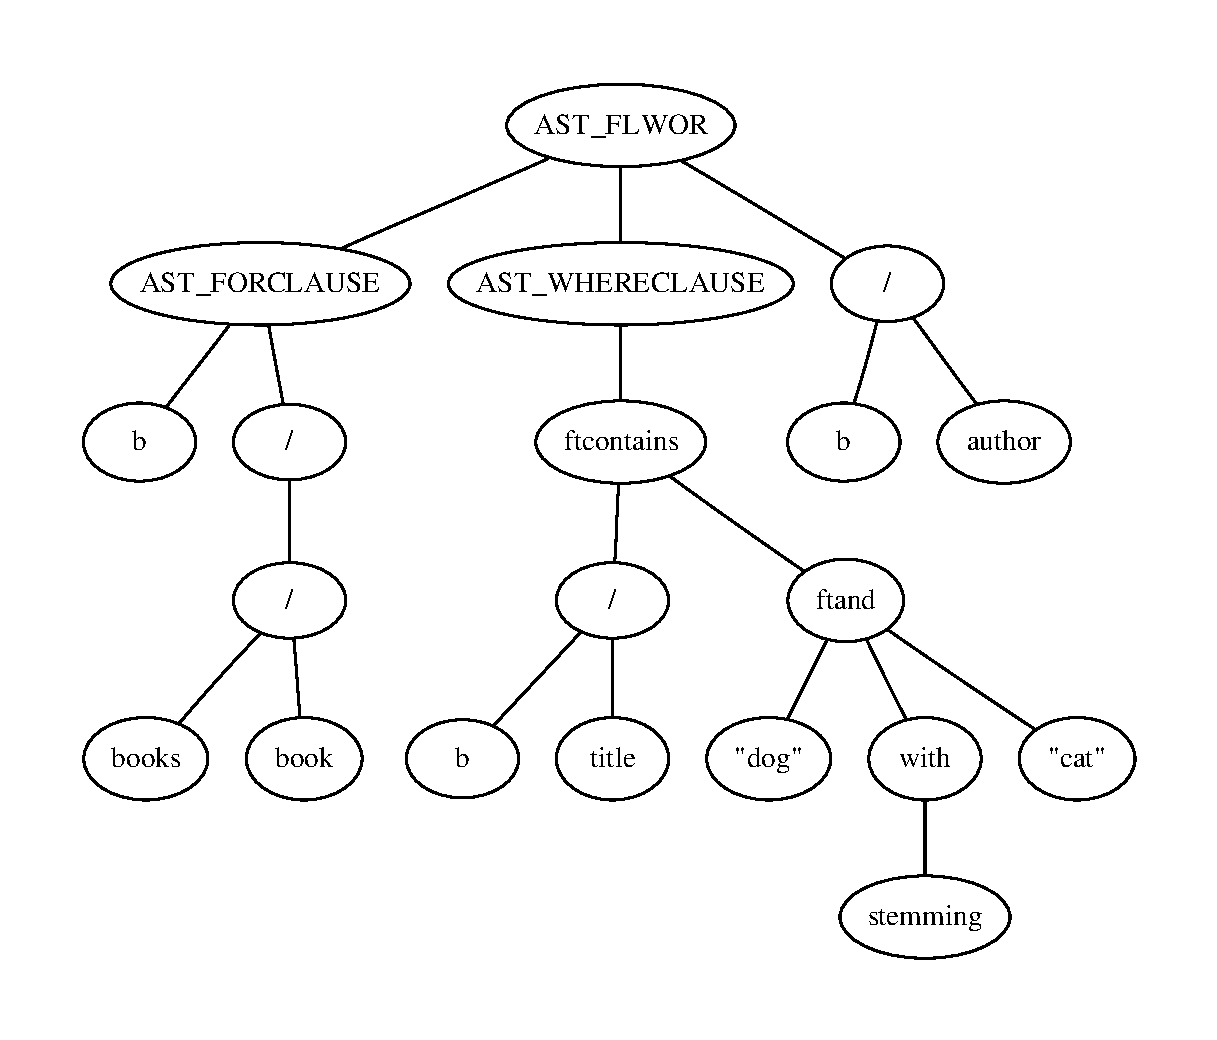
\includegraphics[scale=0.6]{img/graphs/ftq1}
\caption{Generated AST tree for the full-text example in figure \ref{tree:ast:ftq1}}
\label{tree:ast:ftq1}
\end{figure}